\begin{hyperbolicbox}{The action of $\operatorname{PSL}(2,\Z)$ on $\H$}
        \small

        \begin{defi}
            Let $\H$ denote the upper half of the complex plane:
            $$
            \H=\set{z\in\C:\Im z>0}
            $$
            Let $\operatorname{SL}(2,\Z)$ denote the group of matrices of $\Z^{2\times 2}$ with determinant $1$. We define $\operatorname{PSL}(2,\Z)=\operatorname{SL}(2,\Z)/\set{\pm I}$. For each $M=\begin{pmatrix}
                a&b\\c&d
            \end{pmatrix}\in\operatorname{PSL}(2,\Z)$, it acts on $\H$ via the corresponding M\"obius map:
            $$
            z\mapsto\frac{az+b}{cz+d}
            $$
        \end{defi}

        \begin{thm}
            $\operatorname{PSL}(2,\Z)$ is generated by the M\"obius maps $z\mapsto z+1$ and $z\mapsto-1/z$.
        \end{thm}
        \begin{proof}
            Let
            $$
            T=\begin{pmatrix}
                1&1\\0&1
            \end{pmatrix}\aand
            S=\begin{pmatrix}
                0&-1\\1&0
            \end{pmatrix}
            $$
            be the matrices corresponding to $z\mapsto z+1$ and $z\mapsto-1/z$, respectively.
            
            For any matrix $M=\begin{pmatrix}
                a&b\\c&d
            \end{pmatrix}\in\operatorname{PSL}(2,\Z)$. If $\abs{a}\geq\abs{c}>0$, there exists unique $k,r\in\Z$ such that $a=kc+r$ where $0\leq r<\abs{c}\leq\abs{a}$. It follows that 
            $$
            \begin{pmatrix}
                a&b\\c&d
            \end{pmatrix}=
            T^k\begin{pmatrix}
                r&b-kd\\c&d
            \end{pmatrix}
            $$
            If $\abs{c}>\abs{a}>0$, there exists unique $k,r\in\Z$ such that $c=ka+r$ where $0\leq r<\abs{a}$. It follows that
            $$
            \begin{pmatrix}
                a&b\\c&d
            \end{pmatrix}=
            S\begin{pmatrix}
                c&d\\-a&-b
            \end{pmatrix}=
            ST^{-k}\begin{pmatrix}
                r&d-kb\\-a&-b
            \end{pmatrix}
            $$
            Repeatedly apply the two steps above, which will terminate in a finite number of times since $\abs{a}$ decreases each time. $M$ then equals a combination of $T,S$ and a matrix with $a=0$ or $c=0$, which is obviously generated by $T$ and $S$. We conclude that $M\in\group{T,S}$ and then $\group{T,S}=\operatorname{PSL}(2,\Z)$.
        \end{proof}

        \begin{defi}
            By a \textit{fundamental domain} for $\H/\operatorname{PSL}(2,\Z)$ we mean an open subset $\mathcal{F}\subset\H$ where $\mathcal{F}\cap\gamma\mathcal{F}=\emptyset$ for $\gamma\in\operatorname{PSL}(2,\Z)\setminus\set{I}$ and $\bigcup\gamma\closure{F}=\H$.\cite{milneMF}
        \end{defi}
        \vspace{-1em}
        
        Figures below visualize the action of $\operatorname{PSL}(2,\Z)$ on $\H$ and the standard fundamental domain $\mathcal{F}$ (shaded area) given by

        $$
        \mathcal{F}=\set{z\in H:\abs{\Re z}<\frac{1}{2},\abs{z}> 1}
        $$  
        
        \begin{figure}[H]
            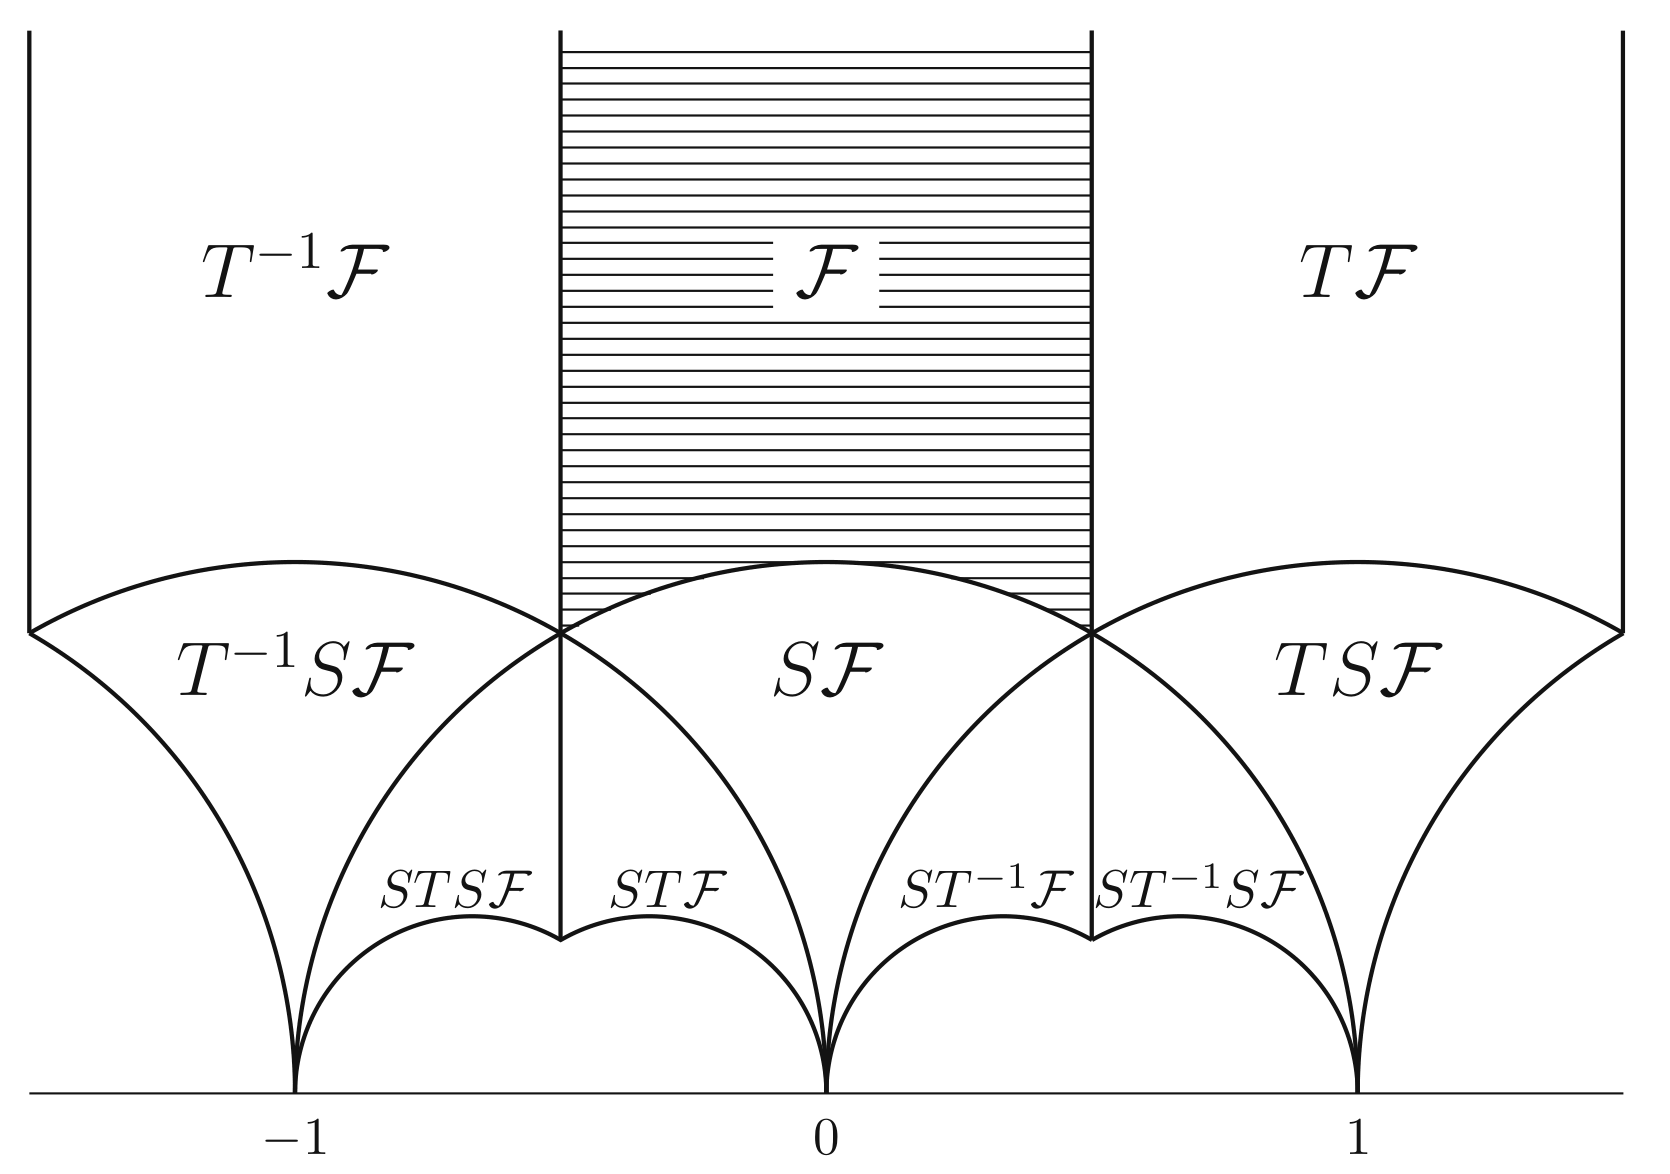
\includegraphics[width=0.4\linewidth]{Images/fund1.png}
            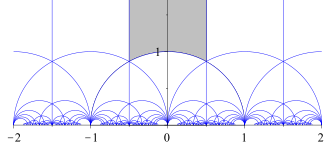
\includegraphics[width=0.55\linewidth]{Images/fund2.png}
        \end{figure}
        
        Each hyperbolic triangle in the images can be translated from the fundamental domain via a M\"obius map in $\operatorname{PSL}(2,\Z)$.
    \end{hyperbolicbox}